\documentclass[11pt]{article}

\usepackage[margin=2.5cm]{geometry}
\usepackage{tcolorbox}
\usepackage{booktabs}
\usepackage{graphicx}
\usepackage{float}
\usepackage{verbatim}

\begin{document}

\title{Assignment 2: Constraint Satisfaction Problems}
\author{Anders Emil Bergan \& Jens Martin Jahle}
\date{\today}
\maketitle


\tcbsubtitle{Sudoku boards solved}

\begin{figure}[H]
    \centering
    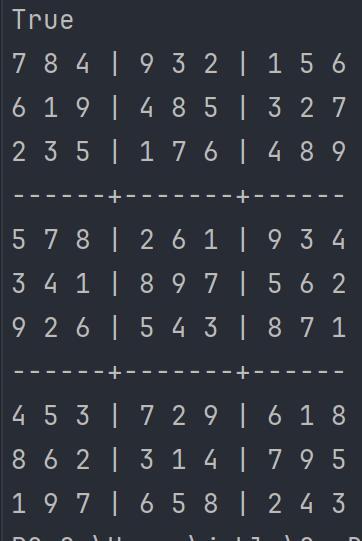
\includegraphics[width=0.6\textwidth]{images/sudoko_easy}
    \caption{Sudoku solution — Easy}
\end{figure}

\begin{figure}[H]
    \centering
    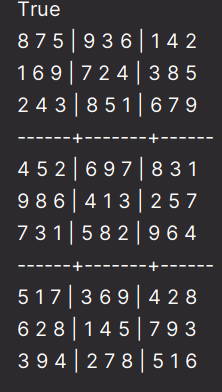
\includegraphics[width=0.6\textwidth]{images/sudoko_medium}
    \caption{Sudoku solution — Medium}
\end{figure}

\begin{figure}[H]
    \centering
    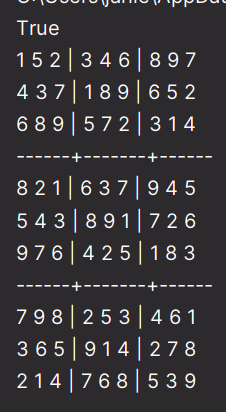
\includegraphics[width=0.6\textwidth]{images/sudoko_hard}
    \caption{Sudoku solution — Hard}
\end{figure}

\begin{figure}[H]
    \centering
    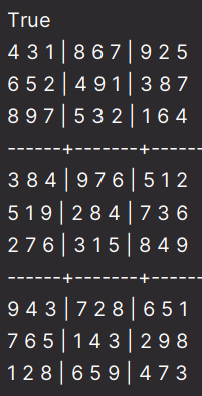
\includegraphics[width=0.6\textwidth]{images/sudoko_very_hard}
    \caption{Sudoku solution — Very Hard}
\end{figure}

\tcbsubtitle{Results}

\subsection*{Summary Table}
\begin{table}[H]
\centering
\begin{tabular}{lrrrrr}
\toprule
Board & BT Calls & BT Failures & AC-3 (s) & BT (s) & Total (s) \\
\midrule
easy & 88 & 6 & 0.015711 & 0.002986 & 0.018698 \\
medium & 292 & 210 & 0.014703 & 0.006203 & 0.020907 \\
hard & 1288 & 1206 & 0.014781 & 0.057230 & 0.072011 \\
very hard & 14382 & 14300 & 0.022067 & 0.577510 & 0.599577 \\
\bottomrule
\end{tabular}
\caption{Backtracking statistics and runtimes per board.}
\end{table}


\section*{Domains after AC-3}

\subsection*{Easy}
\begin{verbatim}
X11: {7,8}
X12: {7,8}
X14: {7,9}
X26: {5,8}
X31: {2,7}
X32: {3,7}
X35: {2,7}
X36: {2,6}
X41: {5,7,8}
X42: {7,8}
X43: {7,8}
X44: {2,5}
X46: {1,2,5}
X61: {5,9}
X64: {3,5,9}
X66: {3,5}
X74: {2,7}
X75: {2,7}
X81: {1,2,8}
X82: {1,6,8}
X83: {2,8}
X84: {2,3,6}
X85: {1,2}
X91: {1,7,8}
X93: {7,8}
X94: {3,6,7}
X96: {1,3,6,8}
X99: {3,4}
\end{verbatim}

\subsection*{Medium}
\begin{verbatim}
X11: {2,5,8}
X12: {2,5,7}
X13: {5,7}
X17: {1,5}
X19: {2,5}
X22: {5,6}
X27: {3,5,6}
X29: {5,6,8}
X31: {2,3,4,6}
X32: {2,4,6}
X33: {3,4}
X37: {3,6}
X39: {2,6,9}
X41: {4,5}
X42: {4,5}
X71: {2,4,5}
X73: {4,5,7}
X77: {4,5}
X78: {2,8}
X79: {2,5,8}
X81: {2,6}
X82: {2,6}
X84: {1,2}
X88: {1,2,8,9}
X91: {2,3,4,5,6}
X93: {3,4,5}
X94: {1,2}
X97: {1,4,5,6}
X98: {1,2}
X99: {2,5,6}
\end{verbatim}


\subsection*{Hard}
\begin{verbatim}
X12: {3,5,6,8}
X14: {3,9}
X16: {6,9}
X17: {6,8}
X18: {5,6,8,9}
X21: {3,4,6}
X22: {3,5,6,7}
X23: {3,4,5,7}
X24: {1,2,3,7,9}
X26: {1,2,6,9}
X27: {1,2,6}
X28: {1,5,6,9}
X29: {1,2,5}
X31: {6,8}
X32: {6,7,8}
X35: {2,7}
X36: {1,2,6}
X38: {1,6,8}
X41: {3,8}
X42: {1,2,3,8}
X43: {1,3}
X45: {2,3}
X48: {1,3,4,5,8}
X49: {1,3,5,8}
X53: {1,3,7}
X54: {1,3,8,9}
X55: {3,9}
X56: {1,8,9}
X57: {1,7,8}
X61: {3,8,9}
X62: {1,2,3,7,8,9}
X65: {2,3,9}
X67: {1,7,8}
X68: {1,3,7,8}
X69: {1,3,8}
X72: {1,5,6,9}
X74: {2,9}
X75: {2,5,9}
X78: {1,6}
X79: {1,2}
X81: {3,4,6,9}
X82: {3,5,6,9}
X83: {3,4,5}
X84: {2,7,8,9}
X86: {2,4,8,9}
X87: {2,6,7,8}
X88: {3,6,7,8}
X89: {2,3,8}
X92: {1,3}
X93: {1,3,4}
X94: {7,8}
X96: {4,8}
X98: {1,3,7,8}
\end{verbatim}


\subsection*{Very Hard}
\begin{verbatim}
X11: {4,5,8,9}
X12: {2,3,4,5,9}
X14: {2,5,6,8,9}
X15: {5,6,8,9}
X17: {5,8,9}
X18: {2,8,9}
X19: {2,5,8,9}
X22: {2,5,9}
X23: {2,5,7,9}
X25: {5,8,9}
X26: {1,2,8}
X28: {1,2,7,8,9}
X29: {2,5,7,8,9}
X31: {5,8,9}
X32: {2,5,9}
X33: {2,5,7,9}
X34: {2,5,8,9}
X36: {1,2,8}
X37: {1,5,7,8,9}
X43: {4,5,9}
X44: {2,9}
X47: {1,4,5,9}
X48: {1,2,4,9}
X49: {2,5,9}
X51: {1,4,5,9}
X52: {1,4,5,9}
X53: {4,5,9}
X54: {2,8,9}
X55: {4,8,9}
X56: {2,4,8}
X57: {1,4,5,7,8,9}
X63: {4,6,9}
X64: {3,8,9}
X67: {4,8,9}
X68: {4,8,9}
X69: {8,9}
X71: {4,9}
X72: {3,4,6,9}
X73: {3,4,6,9}
X74: {3,6,7,8}
X76: {3,4,8}
X77: {4,6,7,8,9}
X82: {3,4,5,6,9}
X83: {3,4,5,6,9}
X85: {4,5,6,8}
X86: {3,4,8}
X88: {4,8,9}
X89: {3,8,9}
X91: {1,4,5}
X92: {1,2,3,4,5,6}
X94: {3,5,6,7}
X95: {4,5,6}
X97: {4,6,7}
X98: {4,7}
X99: {3,7}
\end{verbatim}


\section*{Discussion}
What stands out most from these experiments is how much AC-3 can simplify the problem before backtracking even starts.
On the \emph{easy} and \emph{medium} puzzles, AC-3 was able to cut down the possibilities so well that most cells were already fixed or had very few options left.
Because of that, the backtracking phase felt almost effortless, only a handful of calls, hardly any failures, and the solutions came out almost instantly.

The story is very different once we move to the \emph{hard} and \emph{very hard} puzzles.
Here AC-3 still does some useful pruning, but many cells keep several candidate values.
That leaves the backtracking search with a lot more guessing to do, and we can see this clearly in the numbers: thousands more calls and failures, and runtimes that are orders of magnitude higher.
This shows the limits of AC-3: it only makes the puzzle locally consistent, but it can’t see the deeper patterns that only appear when the solver actually tries out assignments.

If we look at the runtimes overall, we see that AC-3 dominates the easier puzzles, while backtracking dominates the harder ones.
Still, combining them is a big win compared to using backtracking alone.
By cleaning up the obvious conflicts first, AC-3 makes sure the search doesn’t waste time exploring dead ends.

Looking ahead, there are plenty of ways this solver could be made smarter.
Right now it just picks variables and values in a simple order, without any particular strategy.
If we gave it a bit more guidance, for example by choosing the variable with the fewest remaining options or the value that rules out the least for the others, the search would likely become much faster.
We could also add extra inference, such as forward checking, to rule out bad choices earlier.
These changes would not make much of a difference on the easy puzzles, since those are already solved almost instantly, but they could save a lot of work on the hard and very hard ones.

\end{document}
